\documentclass{article}

% Language setting
% Replace `english' with e.g. `spanish' to change the document language
\usepackage[english]{babel}

% Set page size and margins
% Replace `letterpaper' with `a4paper' for UK/EU standard size
\usepackage[a4paper,top=2cm,bottom=2cm,left=3cm,right=3cm,marginparwidth=1.75cm]{geometry}

% Useful packages
\usepackage{amsmath}
\usepackage{graphicx}
\usepackage[colorlinks=true, allcolors=blue]{hyperref}

\title{TDT4171 — Artificial Intelligence Methods \\ Assignment 8 - Deep Learning}
\author{Erik Storås Sommer - 535006}
\date{March 2023}

\begin{document}
\maketitle
\setlength{\parindent}{0pt}

\section*{Intro}

In this assignment a feedforward and a recurrent neural network is implemented and trained using keras. 
I have testet several different architectures and hyperparameters, and the best performing model is presented in this report.

\subsection*{Feedforward Neural Network}

\begin{figure}[hbtp]
    \centering
    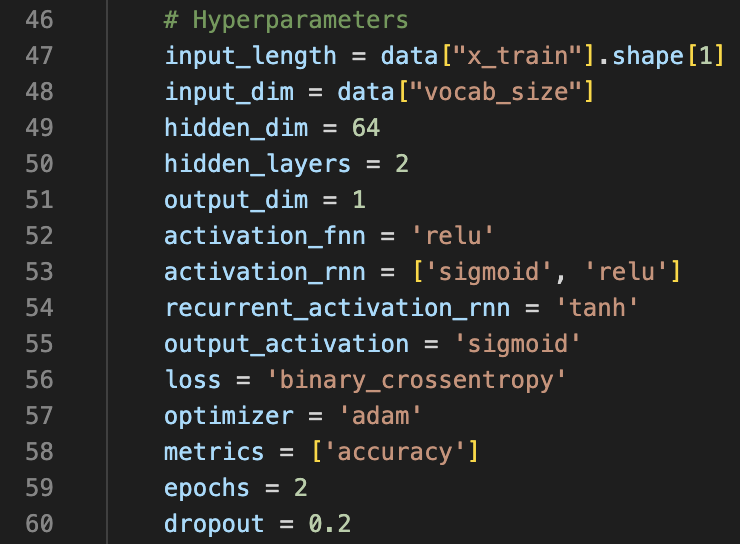
\includegraphics[width=0.8\textwidth]{hyperparameters.png}
    \caption{Hyperparameters used for the neural network}
    \label{fig:image1}
\end{figure}


\begin{figure}[hbtp]
    \centering
    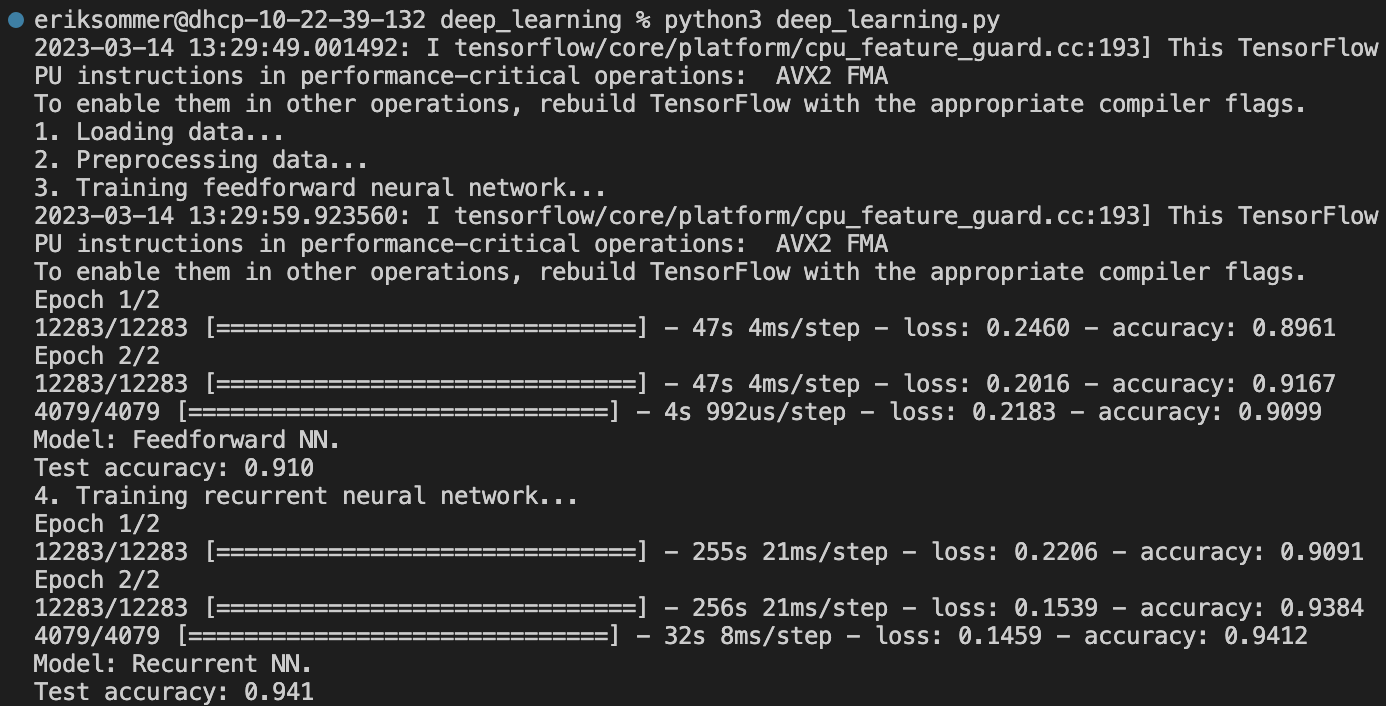
\includegraphics[width=0.8\textwidth]{output.png}
    \caption{Output from running the attached python file}
    \label{fig:image2}
\end{figure}

\end{document}